\chapter{X-ray Diffractometers}

As this chapter will explore, powder diffractometers have been around for a long time, but in recent years both commercial lab instruments and in particular synchrotron instruments have advanced dramatically. 
Historically, there were two approaches used for measurement of diffraction using an x-ray tube source. 

\section{Debye-Scherrer}
The original Debye-Scherrer camera\index{Debye-Scherrer geometry} placed a sample into a capillary tube and a ring of x-ray sensitive photographic film was placed around the sample. (The film needed to be loaded in a darkroom, as light would fog the film.) A measurement was made over hours or days and then the film was taken to a darkroom and developed. To convert to a pattern showing intensity vs. angle, a photo-densitometer was used to measure the darkness of the film. The collimation of the x-ray source and the size of the sample dictated the width of peaks on the film, which in general was not very good. A later development (1937) was the Guinier camera, which used a focusing monochromator to improve the resolution significantly. To this day, Debye-Scherrer geometry is used to describe this setup, where a capillary sample is placed in an x-ray or neutron beam. Since the beam must transverse some part of the sample to be observed (the amount varies with angle), this is also called transmission mode diffraction. The beam is larger than the width of the sample, so that the sample is fully illuminated. Diffracted radiation can be measured in a number of ways: 
\begin{itemize}
    \item 
With a discrete detector that is scanned to give a measurement as a function of angle. With synchrotrons, 
a perfect-crystal monochromator (crystal analyzer) is usually placed in front of the discrete detector, which tightly limits the angular acceptance range for the detector and strongly restricts the observed wavelength range. Recent work replaces the discrete detector with an area detector. The use of a post-sample monochromator provides for very high resolution and very low background levels. Multiple detectors are commonly used, as this type of measurement otherwise is very slow. 
\item
With a linear position-sensitive detector (PSD)\index{position-sensitive detector}\index{PSD} that measures many angles at a time, which may be scanned if the total angular range is small; These measurements can be very fast and have good resolution, but do not reject fluorescence and have have poorer collimation than post-sample monochromation leading to higher backgrounds. 
\item 
With a two-dimensional detector, which technology limits to almost being always flat, though curved would be preferred. The resolution is dictated by the size of the sample, the number of pixels in the detector, and the distance between the sample and detector. Count rates are faster than PSD's, but collimation is even more poor. Count times are frequently seconds with a lab source and fractions of a second with a synchrotron. 
\item
Film is pretty much a thing of the past. This is a good thing as it was very difficult to linearize the intensity scale from film. 
\end{itemize}

A significant limitation of the Debye-Scherrer geometry is that if the sample absorbs appreciably (or scatters an appreciable fraction of the incident radiation in modes other than diffraction) then much of the scattering intensity will be lost. That amount depends on angle, so when there is significant intensity loss, this must be incorporated into the data reduction or fitting as an absorption correction. This is discussed further in \S\ref{ref:Absorption}.

It should be noted that the assumption is that the sample is placed exactly at the middle of the detector rotation circle. Any deviations from this produce a distortion between the measured $2\theta$ angle and the actual diffraction angle. This must be compensated for in fitting, as will be discussed later in \S\ref{ref:SampleDisplacement}.

The original Debye-Scherrer cameras used a small motor to rotate the capillary along its long axis. This is still commonly done in Debye-Scherrer geometry measurements as it brings two advantages. First, it increases the effective number of crystallites that contribute to scattering. This is because a crystallite must be properly oriented with the beam and detector for diffraction to occur. By rotating the sample along an axis, one of the degrees of freedom in this alignment problem will always be satisfied and many more crystallites are now able to contribute to the pattern. This reduces the size of a sample that is needed to produce an accurate diffraction pattern significantly. The second improvement has to do with texture. If crystallites are placed into the capillary in a non-random way, the rotation will raise the symmetry of the texture, where the only possible orientational ordering would be along the capillary direction; this is called cylindrical texture. 

Related to the Debye-Scherrer camera is a device that spins the sample on two different axes. This is known as a Ganolfi camera.\index{Ganolfi camera} It takes some care to design the spinning so that it performs the closest thing possible to optimal randomization in a non-random process and can produce a powder diffraction pattern from a single-crystal specimen. 

\section{Bragg-Brentano Diffractometer}\label{ref:Bragg-Brentano}
The concepts behind the Bragg-Brentano diffractometer\index{Bragg-Brentano diffractometer} were developed in the 1920's by J. C. M. Brentano\index{Brentano, J.} while working in the laboratory of Laurence Bragg\index{Bragg, W. L.}, as an advance over ideas from H. Seemann\index{Seemann, H.} and H. Bohlin\index{Bohlin, H.} but was first produced as a working instrument in the 1940s. A very successful commercial Bragg-Brentano instrument was developed in the early 1950's by William Parrish\index{Parrish, W.} for Norelco. 
The concept for this type of instrument is outlined in Fig. \ref{fig:BraggBrentano}. 
To explain this concept, as x-rays leave the x-ray tube, they will spread in all directions, but slits and shielding limit the x-rays to diverge along a fixed angular range. 
The x-rays that impinge on the sample are diffracted back towards the detector, if the Bragg diffraction condition is satisfied, with slits used to prevent x-rays from other paths from reaching the detector.
Thus, the loss of intensity from the spread of x-rays leaving the x-ray tube is partially offset by this parafocusing\index{parafocusing}.  
It is called parafocusing, rather than focusing, because the focusing condition would only be satisfied if the sample were to be curved along the outlined focusing circle, as this would focus the point source of x-rays back onto the detector, but this is only approximated by a flat plate. As shown in the figure, this curvature would have to change with $2\theta$ because the radius of the focusing circle changes as $2\theta$ changes so creating a curved sample is never attempted. Note that one other effect of changing $2\theta$ is that the length that the x-ray source projects onto the sample changes. This length is determined by slits that transmit a fixed divergence angle. The illuminated length becomes longer at lower $2\theta$. 
\begin{figure}
    \centering
    \begin{subfigure}{0.49\textwidth}
        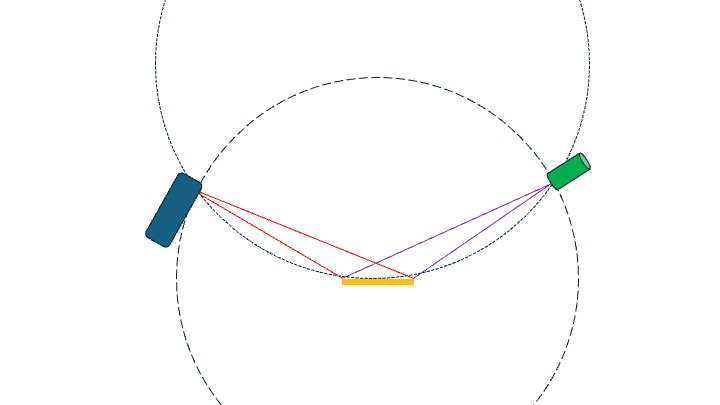
\includegraphics[width=0.9\linewidth]{figures/BraggBrentano1.jpeg}
        \caption{Lower $2\theta$ setting}
    \end{subfigure}
    \begin{subfigure}{0.49\textwidth}
        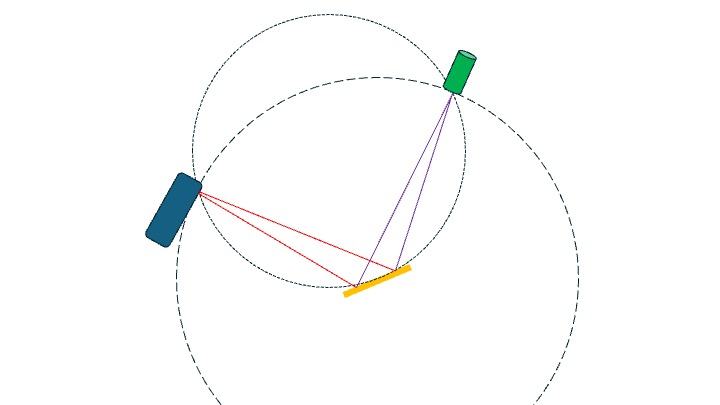
\includegraphics[width=0.9\linewidth]{figures/BraggBrentano2.jpeg}
        \caption{Higher $2\theta$ setting}
    \end{subfigure}
    \caption{Schematic representation of a Bragg-Brentano parafocusing x-ray diffractometer with two angular settings. The blue object represents the x-ray tube; the green cylinder the detector; the yellow rectangle is the sample. The red lines outline the projection of x-rays onto the sample, while the purple lines show the allowed path for x-rays to reach the detector. The dotted-line circle, (running through the source, sample and detector), is the focusing circle and the dashed-line circle that is centered on the sample is the $2\theta$ circle. Note that the size of the focusing circle and the length of illuminated sample both decrease at the higher $2\theta$ setting.}
    \label{fig:BraggBrentano} 
\end{figure}
There are two variations on this diffractometer. In the example shown in Fig. \ref{fig:BraggBrentano}, the detector rotates around the $2\theta$  circle and the sample rotates at half the angle of the detector. This is called a in a $\theta$-$2\theta$ diffractometer. In the less common and more expensive $\theta$-$\theta$ diffractometer, the detector and x-ray source both rotate around the $2\theta$ circle and the sample remains stationary.

An alternative to Bragg-Brentano geometry is the related Seemann-Bohlin diffractometer. 
Here, the x-ray tube and the detector not only rotate but also move towards and away from the sample to keep the focusing circle radius constant. 
This allows the sample to be curved along that fixed radius so that the ideal focusing condition is met, but this requires an exceedingly complex mechanical design with relatively minor gain. 
I have never seen a Seemann-Bohlin diffractometer in use. 

Since the x-ray beam travels through the sample only as far as need be before it is diffracted, this geometry is called reflection mode diffraction. 
Note that the $2\theta$ angle drops close to 0, the x-ray beam becomes close to parallel to the sample surface. This has two experimental implications. 
One is that if the sample is not perfectly smooth, the diffraction intensities become reduced as a result of surface roughness. 
The second is that the distance the x-ray beam penetrates into the bulk of the sample decreases with $2\theta$. This produces a slight but perceptible shift in the effective sample position, in an effect known as sample transparency\index{sample transparency}\label{sample transparency}. 
The sample must be sufficiently thick so that at the highest measurement angle, no significant amount of x-rays will travel completely through the sample and will be lost. 
When this is true, diffraction intensities do not need to be corrected for sample absorption.  
There is no easy way to correct the intensity loss when samples are not sufficiently thick, but note that this would only be a problem for very low density materials or very thin samples. With highly absorbing samples, a different problem can arise. Only the very top of the sample is probed by the x-ray beam. The particles at the top may not be representative of the bulk with respect to composition, morphology or phase abundance. 

The slits that define the angular range that determines the portion of the sample that is illuminated should be set so that at the lowest diffraction angle to be used, the x-ray beam does not extend past the sample. 
An alternative to this is to have the instrument adjust the slits defining the beam path to have the same length independent of $2\theta$, this is known as $2\theta$-compensating slits.\index{ $2\theta$-compensating slits} 
Traditionally, use of  $2\theta$-compensating slits for Rietveld analysis is considered a bad idea, as the diffraction intensities must be scaled for the changing illumination range. 
With modern, highly computerized, diffractometers, I'm not so sure that it is not better to have the same region of sample used for all measurements, even though, as noted, the exact crystallites that will contribute to the pattern will still change as the amount that the x-ray beam penetrates into the sample decreases with angle. 

It is common to use a sample holder for Bragg-Brentano diffraction consisting of a single crystal (typically sapphire) that is cut so that diffraction from this crystal will never occur when the crystal is mounted along the diffraction circle. It is then possible to measure a diffraction pattern from a small amount of sample placed on this so-called ``zero background'' sample mounting. While this is a good method for measuring a diffraction pattern with a small amount of sample, the diffraction intensities will have the same deviations from correct as a thin sample and should not be used for Rietveld analysis. That small amount of sample can be used for an accurate powder diffraction pattern if placed in a capillary tube and used in a transmission experiment, particularly if the capillary is spun. It is also common to spin samples in a Bragg-Brentano instrument. However, this type of spinning is done around the normal to the plane of the sample, which does not bring new crystallites into an orientation that allows diffraction. This does not improve the particle counting statistics; Bragg-Brentano sample-spinning is done to simplify possible texture, but forcing it to have cylindrical symmetry, if present. It is possible to oscillate a sample in a Bragg-Brentano diffractometer to improve particle counting statistics, but this must be done by increasing and decreasing the sample angle (properly this rotation of the $\omega$ axis, but more commonly the angle is called $\theta$) or with an oscillation  perpendicular to the $2\theta$ circle. Neither is commonly done, as it interferes with parafocusing. 

In Bragg-Brentano diffraction, the assumption is that the sample is placed exactly at the plane of the diffractometer circle with accuracy better than a fraction of a micron. This cannot be achieved routinely (a human hair is 50-100 microns) and must be corrected for in fitting, as it produces a slight but significant deviation between the measured $2\theta$ angle and the actual diffraction angle. A second correction is important for samples that are of low density. As noted, the amount the x-ray beam penetrates into the sample changes with $2\theta$\index{sample displacement} and for low density samples this affects the apparent location of the sample due to sample transparency and again this must be corrected\index{sample transparency}. Both corrections will be discussed later in \S\ref{ref:SampleDisplacement}.

\section{Synchrotron-based instrumentation}
Synchrotrons were originally developed for research using the electron beams that they contain, and the x-ray radiation they generated was  considered a nuisance. Eventually, scientists started using larger synchrotrons for the highly collimated x-ray beams that they produce during hours when the beams were not being used for research. The second generation of synchrotrons were built specifically as x-ray sources, primarily using bending magnet sources, which produce a broad wavelength spectrum with a fairly large source effective source size. The third generation of synchrotrons were built around use of insertion devices, that produce a strongly-peaked x-ray spectrum and have a much smaller source size. The fourth generation of synchrotron sources reduce the size of the x-ray beam considerably generating even smaller effective source sizes from insertion devices and much higher coherence in the x-ray beams. The coherence is of no advantage for powder diffraction, but the small source size of insertion devices, particularly at 4th generation sources, is definitely beneficial to design of powder diffraction instrumentation. 

There is a plethora of designs for synchrotron powder instruments, but nearly all use a double-bounce incident-beam monochromator, where the x-ray beam is diffracted from two perfect crystals to remove all but one precise wavelength of x-rays from the beam. Since perfect crystals are used, the wavelength spread is very small, which in turn allows for very high resolution instruments. While a survey of the different types of synchrotron instruments across the world would itself make for an interesting book, I will attempt to categorize them here. 
\subsection{Ultra-high resolution instruments} These instruments place a perfect-crystal monochromator between the sample and the detector. This analyzer creates an instrument that has excellent signal-to-noise as the monochromator will only transmit x-rays that have precisely the right wavelength and originate from the right location it will also have very narrow peak widths, limited usually by the performance of the sample. The analyzer detector is superb at rejecting fluorescence and the very limited angular acceptance of the perfect crystal creates a parallel-beam optic that means that a larger sample size does not degrade resolution. The advantages of a perfect-crystal analyzer were demonstrated by Dave Cox at Brookhaven National Lab in the 1980's.\index{Cox, D.} and it was he who constructed the first dedicated powder instrument of that type at Brookhaven's NSLS source. The downside of use of three crystals in the beamline optics is that only a very small fraction of the photons from the source can be used for measurements and most ultra-high resolution powder diffractometers use multiplexed detectors to speed their measurements. In such instruments data collection speeds are typically in the range of 10 minutes to an hour. The monochromator-detector assembly is quite massive and these instruments are quite large and expensive. 

\subsection{Linear PSD diffraction} It is possible to make detectors that will record the position of an incident photon along the length of the detector. Hence they are known as linear position-sensitive detectors. They may be flat or curved. It is now possible to build an instrument that covers the entire angular range for measurement with no gaps, but older designs did leave gaps and the detector would need to be rotated in order to collect an entire pattern. 

Linear PSDs can be constructed with very high angular detection precision, so their angular resolution can come close to that of the ultra-high resolution instruments with perfect-crystal analyzers, but the resolution depends on having a very small sample. The larger the sample, the more the uncertainty in where the x-ray originated, which directly translates to wider peaks. Linear detectors may have the ability to electronically filter out some fluorescence but are not as effective as a perfect-crystal analyzer and will also count any photon that reaches the detector regardless of the angle of origin, so they are not as good at rejecting air scattering and other sources of stray photons, such as scattering from slits, furnaces and refrigerators, so linear PSD instruments will have significantly higher backgrounds than ultra-high resolution measurements, but will be much faster: seconds to minutes. The as the resolution of the linear detector dictates the ultimate resolution, there becomes a tradeoff between angular range coverage, resolution and cost for the instrument. The size is quite variable across institutions but these instruments are in general quite expensive. 
\subsection{Area detection instruments} Initially, electronic area detectors for x-rays were developed as a replacement for x-ray film in medical procedures and for this we can be very thankful as it significantly reduced the amount of x-rays that we needed to be exposed to for medical and dental diagnosis. These detectors were valuable for diffraction instrumentation, but since that time, detectors that are more specialized for x-ray science have been developed. These detectors are faster in their readout times, have progressed towards smaller pixels and to larger sizes. The fastest detectors with the largest numbers of pixels can alone cost millions of dollars. 

Area detection has revolutionized powder diffraction measurements for pair distribution function (PDF) determination\index{pair distribution function}\index{PDF}. These require a short x-ray wavelength to obtain patterns collected over a very wide Q range. The work of Pete Chupas\index{Chupas, P.} and others showed that with an area detector placed close to a sample, one could collect a full pattern for a PDF in seconds rather than take scans that took a large fraction of a day for a single PDF. Likewise, while I used a point detector for single-crystal diffraction in my student days, I do not think that anyone would consider using a point detector for this in the current century. Area detectors provide the most efficient diffraction measurements as the capture the greatest solid angle of scattering from the sample, so count rates are exceedingly high; measurements can be as quick as the detector electronics allow. There is typically no collimation possible between the sample and detector, so backgrounds can be quite high. 

The resolution possible with an area detector is determined by the size of the sample, the pixel size of the detector, relative to the distance between the sample and the detector so there is a playoff between angular range and resolution for a particular size of detector, which is why larger and higher pixel density detectors are preferred. Powder diffraction usually does not demand the highest detector readout rates needed for many other techniques. My personal thinking is that while PSD-based instruments provide the most convenient data collection, an area detector instrument can offer equivalent resolution and much faster data collection. Having been involved with ultra-high resolution diffraction since my days with Dave Cox, this is my favorite choice for x-ray diffraction. 

\section{X-ray detection and counting statistics}\label{ref:CountingStatistics}
As was noted, in the early days, x-ray film was one of the primary detection methods for x-rays. Geiger-Müller detectors were also used. These days, most but not all x-ray detectors count individual photons as they hit the detector. There is often some mechanism to filter out events that occur with too little energy (likely noise) or too much energy (cosmic rays) so at least some spurious signals can be removed. Some detectors, such as CCD imaging devices, measure the deposited energy, and do not measure individual photons. It is important to know the difference. In the case of photon counting, one measures discrete events, but one wants to extrapolate that to a rate that photons are arriving on average. The more photons that are counted, the more accurate that rate is known. The uncertainty in this rate is known as Poisson noise or shot noise.\index{Poisson noise}\index{shot noise} and follow rules that are commonly called counting statistics.\index{counting statistics} For larger numbers of counts, say 20, the uncertainty in the rate will be the square root of the number of counts. While this becomes inaccurate for smaller numbers, this is usually ignored. With non-photon counting detectors, the uncertainties in the measurement must be determined from the detector properties. This is not always simple, but is important as the optimum results from fitting are only obtained when observations are weighted properly with respect to their experimental uncertainties. 

\section{X-ray absorption in Debye-Scherrer Geometry}\label{ref:muR}
While x-ray absorption is usually not a problem in Bragg-Brentano measurements, it is crucial that it be considered in the design of a Debye-Scherrer measurement and key to that is knowing the value of $\mu R$, which is a unitless quantity that measures the amount of absorption. 

GSAS-II provides a tool, program Absorb\index{software!Absorb} (see \S\ref{ref:Absorb}) that can be used to determine the linear absorption coefficient, $\mu$, and where $R$ is the radius of the sample capillary. Note that since $\mu$ normally has units of $\rm cm^{-1}$, $R$ must be converted to the \textit{inner radius in cm}, since normally capillary sizes are given as a \textit{diameter in mm}, and often for the outer dimension. In addition to computing $\mu$ and $\mu R$, program Absorb plots the effect of changing the x-ray wavelength and the range for the correction as a function of $2\theta$, which can be useful to consider potential changes to the measurement. 

The effect of absorption on the experiment will depend on the magnitude of $\mu R$, as follows:

 \begin{itemize}
     \item $\mu R < 0.5$: in this range the effect of absorption is quite small and can be ignored. At $\mu R = 0.5$, approximately 50\% of the incident x-ray flux is lost to absorption, but the variation with angle is less than 5\% over the likely range of the experiment and thus is negligible. 
     \item $0.5 < \mu R < 1.0$: In this range, absorption becomes significant, where at $\mu R = 1.0$ as much as 80\% of x-rays are absorbed and the absorption correction can be as large as 20-25\%. However, a rule of thumb developed by Alan Hewat long ago for Debye-Scherrer geometry is that if $\mu R$ is less than 1, the effect of absorption will be a minor perturbation on the ADPs, so unless having an accurate ADP determination is particularly important, an absorption correction can be omitted.  
     \item      $1.0 < \mu R < 1.5$: In this range absorption will significantly degrade reflection intensities, with losses as high as 90\% of x-rays lost to absorption, but the data can be corrected well. If it is possible to reduce the sample diameter to bring $\mu R < 1$, this would improve the experiment. If not, an absorption correction is necessary to obtain accurate results as it can change the measurements by nearly a factor of 2.
     \item $1.5 < \mu R < 2.5$: At this point absorption now is quite severe. Even at high angles (where losses are least desirable) the vast majority of the incident beam is lost. This can be successfully corrected, but this is less than ideal. Plan to increase counting times by as much as an order of magnitude over what would normally be required. Consider the options in the next section as alternatives. 
     \item $2.5 < \mu R$: Under normal circumstances, these measurements are not successful. Some people will consider making a measurement with $\mu R < 5$ if the result is sufficiently valuable to afford the measurement time. There are a number of options that should be considered to reduce the sample absorption: 
     \begin{itemize}
         \item if near an element's absorption edge, use a different wavelength, if not near an edge, decrease the x-ray wavelength;
         \item consider using a smaller diameter capillary;
         \item consider diluting the sample, either with a small unit cell crystalline material that will add only a small number of peaks (diamond powder?) or a low-density non-crystalline phase (amorphous boron?). 
     \end{itemize}
 \end{itemize}

If you are performing an experiment with a highly absorbing sample, you are recommended to measure a good estimate for the packed density of the actual specimen you are using for the measurement. This can be done by weighing the capillary before filling it and again after filling it. This will require a balance with microgram sensitivity. In addition, estimate the length and inner diameter of the region filled with the sample to determine the volume. A microscope can be helpful for this. 

\section{For More Information}

\begin{itemize}
\item 
  \textit{International Tables for Crystallography, Volume H: Powder Diffraction} (2019), edited by C. J. Gilmore, J. A. Kaduk, and H. Schenk, DOI: 10.1107/97809553602060000115
  \begin{quote}
This is a comprehensive reference on powder diffraction. If your library does not have a physical copy of this, they may offer on-line access.
  \end{quote}

\item\textit{Fundamentals of Powder Diffraction and Structural Characterization of Materials} (2025), P. Y. Zavalij and V. K. Pecharsky, Pecharsky \& Zavalij). Springer, DOI: 10.1007/978-3-031-91504-8

\item\textit{Principles and Applications of Powder Diffraction} (2018), A. Clearfield, J. H. Reibenspies and N. Bhuvanesh, Wiley, DOI:10.1002/9781444305487.  

\item\textit{Powder Diffraction: Theory and Practice} (2008), R. E. Dinnebier and S. J. L. Billinge. Royal Society of Chemistry.
DOI: 10.1039/9781847558237-FP011
\begin{quote}
Any of the above three provide a comprehensive introduction to powder diffraction, with the first two books more aimed at introductory materials, while Dinnebier \& Billinge is a collection of chapters written by leading researchers.
\end{quote}

\item\textit{X-Ray Diffraction Procedures: For Polycrystalline and Amorphous Materials}, 2nd Edition (1974), H. P. Klug and L. E. Alexander. Wiley. 
\begin{quote}
Quite old and very expensive, but still the best discussion of laboratory instruments to my knowledge. 
\end{quote}

\item
Jeremy Cockcroft\index{Cockcroft, J.} provides notes from an on-line powder diffraction course:
\url{http://pd.chem.ucl.ac.uk/pd/indexnn.htm}

\end{itemize}
